\chapter{Basis SaX2 Workflow (X11 R6 v4.x)}
\label{cha:dsp}
\minitoc
Zur Konfiguration von X11 R6 v4.x wurde ein dreischichtiges Modell
entwickelt. Kurz angesprochen wird in der ersten Schicht eine
Registrierung der Hardware vorgenommen (init). Innerhalb der 
zweiten Schicht erfolgt die Erstellung einer initialen Konfiguration
aus den erkannten Hardwaredaten (xc). Sollte diese Initialkonfiguration
nicht den Anforderungen entsprechen kann in der dritten Schicht
die eigentliche Konfiguration und Testphase beginnen (xapi).

Die Trennung der Konfiguration in drei Layer ist auch Grundlage
um SaX2 in YaST2 integrieren zu k"onnen. Das Zusammenspiel
der drei Schichten innerhalb von YaST2 ist im Kapitel ~\ref{cha:yst}
n"aher beschrieben. In diesem Kapitel wird das Zusammenwirken von
init, xc und xapi in der urspr"unglichen Form beschrieben.

Als Interface zwischen allen Schichten wird das ISaX Modul
verwendet. ISaX dient im wesentlichen zum Schreiben und Lesen
von X11 Konfigurationen. Es bildet zudem ein einheitliches Interface
zwischen X11 formatierten Konfigurationsdateien sowie den bin"ar
abgelegten automatisch erkannten Konfigurationsdaten und dem
durch YaST2 geforderteten YCP Datenformat.

Die in der dritten Schicht bereitgestellten Daten zur X11 Konfiguration
werden beim Speichern der Konfiguration dem ISaX als so genannte 
Variablen API Datei zur Verf"ugung gestellt. Der ISaX generiert daraus
dann die finale xorg.conf. Das Format und die zur Verfuegung stehenden
Konfigurationsvariablen dieser Variablen API Datei sind im Kapitel 
~\ref{cha:api} beschrieben.

Durch das Drei-Schichtenmodell besteht immer die M"oglichkeit Teile 
der einzelnen Schichten auszutauschen oder geziehlt zu "uberpr"ufen.
Die Wartbarkeit des Gesammtsystems ist damit auch "uber einen l"angeren
Zeitraum gegeben. Aus diesem Grund konnte auch die 
Konfigurationsoberfl"ache zur Integration von SaX2 in YaST2 angepasst 
werden (Qt toolkit), ohne dabei das Gesammtsystem in seiner 
Funktionalit"at zu beinflussen.

\index{init.pl}
\section{Level 1: Init}
\label{sec:le1}
Init wird repr"asentiert durch \textbf{init.pl} und "ubernimmt 
dabei folgende Aufgaben:\\
\begin{itemize}
\item Erstellen der prinzipiellen Datenstruktur und Festlegung
      von Default Einstellungen.
\item Erkennung der Hardware bezogen auf PCI/AGP Graphikkarten 
      Zeigerger"ate, Tastatur und Monitor. Der eigentliche 
      Hardwarescan wird durch einen sysp (System-Profiler)
      Aufruf gestartet. Sysp ist ein eigenst"andiges Programm 
      das seine Funktionalit"at durch einklinkbare Module
      erh"alt die dann wiederum eine bestimmte Aufgabe 
      "ubernehmen k"onnen. Eine Beschreibung der einzelnen sysp 
      Module ist im Kapitel ~\ref{cha:sys} zu finden.
\item Eintragen der Daten in die Hardware-Registry. Mittels der
      Funktionen aus dem perl Modul \textit{AutoDetect.pm} 
      werden die durch sysp gelieferten Informationen in die 
      Datenstruktur eingepflegt. Das Ergebnis aus Defaulteinstellungen 
      und Hardwaredaten entspricht der Hardware-Registry, die
      die Basis zur Erstellung der Initialkonfiguration bildet.
\item Speichern der Registry. Die Registrierungsdaten werden dann 
      in der vorliegenden Form als Bin"arstrom unter 
      \textit{/var/cache/sax/files/config} abgespeichert. 
\end{itemize}

init.pl entscheidet selbst ob sich an der aktuellen Hardware
etwas ge"andert hat und ist damit in der Lage auf neue oder ge"anderte
Hardware zu reagieren. Die Entscheidung ob sich an der Hardware etwas
ge"andert hat oder nicht wird mittels des SaX2 \textbf{hwupdate} tools
getroffen. hwupdate benutzt dazu die libhd Datenbank und vergleicht
die gespeicherte Hardware Information mit der aktuell scanbaren.

\index{xc.pl}
\section{Level 2 (xc) und Level 3 (xapi)}
\label{sec:le2}
xc (X-Configuration) wird repres"antiert durch xc.pl und 
"ubernimmt folgende Aufgaben:
\begin{itemize}
\item Lesen der Hardware-Registry. Das Einlesen der Registry
      erfolgt sehr schnell, da die Daten Bin"ar aber bereits 
      in Form eines Hashes abgespeichert wurden. Die Daten 
      k"onnen dadurch direkt in einen Perl Hash eingelesen und
      weiter verarbeitet werden.
\item Mittels der Funktionen aus \textit{CreateSections.pm} 
      wird dann aus der Hardware-Registry eine erste automatische 
      X11 Konfigurationsdatei erzeugt. Diese Konfiguration wird
      dann verwendet um einen X-Server zu starten falls noch kein
      X-Server gestartet wurde auf den xc zugreifen kann.
\item Ist kein X-Server vorhanden auf den zugegriffen werden kann
      so startet xc einen initialen X-Server, pr"uft ob alle Pakete
      zur Konfiguration der Karte(n) installiert sind und zeigt dem 
      Benutzer eine Message-Box mit dem Hinweis, dass dies eine automatisch
      generierte Konfiguration ist. Der Benutzer hat darauf hin die
      M"oglichkeit diesen Vorschlag zu akzeptieren, das ganze
      abzubrechen oder in den Level 3 (xapi) zu wechseln indem
      er das "Andern der Konfiguration anw"ahlt. Verzweigt er in 
      den Level 3 so bildet die Ausgangsposition zur Konfiguration
      die Initialkonfiguration die durch Level 1 (init) erstellt 
      wurde.
\item Ist bereits ein X-Server aktiv auf den auch zugegriffen werden
      kann so erfolgt nur die Pr"ufung auf das Vorhandensein aller
      wichtigen Pakete und danach wird in den Level 3 (xapi)
      verzweigt. Die Ausgangsposition zur Konfiguration bildet nun
      die aktuelle Konfiguration gemessen am Inhalt der Datei
      \textit{/etc/X11/xorg.conf}.
\item Das Verzweigen in den Level 3 (xapi) bedeutet den Start der 
      graphischen Oberfl"ache. Die Oberfl"ache selbst basiert auf
      den aktuellen Qt Bibliotheken. Je nach dem welche Ausgangsposition
      zur Konfiguration geschaffen werden soll erstellt xapi ein
      set von Dateien die unter \textit{/var/cache/sax/files} abgelegt
      werden und mittels ISaX erstellt wurden. xapi liest dann diese
      Daten ein und bringt sie zur Anzeige. ISaX wird "uber eine
      Option mitgeteilt, dass es entweder die Daten der aktuellen
      Konfiguration oder der hardware Registry ausgeben soll.
      W"ahrend der Konfiguration wird dieses set von Dateien 
      entsprechend modifiziert. Am Ende der Konfiguration werden
      diese Dateien mittels des \textbf{getconfig} Skripts zu einer
      Variablen API Datei zusammengefasst und dem ISaX "ubergeben.
      ISaX erzeugt daraus die finale Konfigurationsdatei die auch
      f"ur einen eventuellen Test der Konfiguration benutzt wird.
      Entscheidet sich der Benutzer f"ur einen Test der Konfiguration
      wird ein neuer X-Server gestartet zusammen mit dem Modeline
      Tuning-Tool XFine2 zur Anpassung der Bild Lage/Gr"osse.
      Speichert der Benutzer diese Konfiguration so wird die
      Variable \textit{ImportXFineCache} in die Variablen API Datei
      eingef"ugt und \textbf{getconfig} erzeugt via ISaX dann erneut 
      die finale Konfigurationsdatei. Das Eintragen der Modeline
      "Anderungen in die Konfigurationsdatei wird dabei auch "uber
      den ISaX gesteuert wobei das XFine2 Modul \textit{XFineControl}
      benutzt wird. Die genaue Funktionsweise zur Erfassung von Modeline
      "Anderungen ist im Kapitel ~\ref{cha:xfi} beschrieben.
\end{itemize}

\index{xw}
\section{XWrapper (xw)}
\label{sec:xw}
Im SaX2 Ablauf gibt es einige Stellen an denen ein, oder ein 
weiterer X-Server gestartet werden muss. Der Start eines neuen 
Server erfolgt immer ueber das \textbf{xw.pl} Programm.
Das Programm war urspr"unglich ein Perl Skript wurde dann aber
durch ein C Programm ersetzt. Der Name \textit{xw} is von \textbf{xw}rapper
abgeleitet worden. Das Programm erf"ullt folgende Aufgaben:
\begin{itemize}
\item Start des X-Server in einem eigenen Prozess. Dabei wird die erste
      Option als Logfile Name interpretiert, die restlichen Optionen 
      werden dem X-Server zugef"uhrt. Der Server wird in einem von
      xw durch fork() erzeugten Prozess gestartet. Die Ausgaben des
      X-Servers im Kindprozess die auf dem STDERR Kanal ausgegeben werden 
      werden durch einen freeopen() Aufruf in das logfile umgeleitet.
      xw selbst ( Vater ) verweilt im Vordergrund und wartet.
\item Erst nach dem Eintreffen des SIGUSR1 Signals welches vom X-Server
      an den aufrufenden Prozess geschickt wird, ist der Server bereit
      zu arbeiten. Trifft das Signal ein, so wird der Vater-Prozess 
      beendet w"ahrend der Kind-Prozess ( X-Server ) weiter arbeitet.
      Die Prozessnummer des Kind-Prozesses wird dabei auf STDOUT
      ausgegeben.
\item Auf dem neu gestarteten Server werden folgende Dienst aktiviert
      \begin{enumerate}
      \item TWM Windowmanager starten
      \item Root-Window Hintergrund auf blau setzen
      \item AccessX starten (Maussteuerung "uber dem Nummernblock)
      \item XBanner SuSE Logo auf jeden screen setzen
      \item XBanner text f"ur nicht prim"are screens setzen
      \end{enumerate}
\end{itemize}

\index{Optionen}
\section{Startupskript}
\label{sec:sta}
Die Koordination der Prozesse \textbf{init.pl}, \textbf{xc.pl/xapi}
erfolgt ueber das Startupskript \textit{sax.sh} welches in 
\textit{/sbin} liegt und zumeist ueber das Wrapper 
Skript \textit{/sbin/SaX2} aufgerufen wird. Der Wrapper 
"ubernimmt dabei folgende Aufgaben:
\begin{itemize}
\item Erzeugung eines sicheren tempor"aren Verzeichnisses durch \textbf{mktemp} 
\item Test auf root Rechte. Ruft ein normaler Benutzer das Programm auf, so
      ist eine Authentifizierung erforderlich. Dies geschieht "uber den 
      xauth Mechanismus "uber das \textit{sux} Kommando oder durch den xhost
      Mechanismus falls sux nicht existiert. In Beiden F"allen ist es 
      erforderlich das root Passwort anzugeben. 
\item Aufruf des eigentlichen SaX2 Startskripts \textbf{sax.sh}
\end{itemize}
Die M"oglichkeit Optionen an das Startupskript zu uebergeben wird 
durch die Summe der Optionen aus init.pl und xc.pl gebildet.
Folgende Optionen sind m"oglich:
\begin{itemize}
\item \verb+-b | --batchmode [Dateiname]+\\
      Durch diese Option wird der sogenannte batch modus aktiviert.
      SaX wird in diesem Fall nicht sofort starten sondern bietet 
      eine interaktive Shell zur Eingabe sogenannter Profildaten
      an. Der Batchmode erlaubt es direkt in den Konfigurationsablauf 
      einzugreifen. Ver"anderungen im batch mode werden auch in der 
      registry abgespeichert.
      Der batch mode verlangt Daten in einem speziellen Format, durch 
      die Eingabe von \textit{help} wird dieses Format kurz 
      beschrieben. Es ist jedoch unerl"asslich zu verstehen welche
      Ver"anderungen wo vorgenommen wurden. 
      SaX kann fuer problematische Karten jeweils ein 
      Profil automatisch zuordnen. Der Inhalt dieser sogenannten
      Profildateien entspricht demselben Format wie es bei der
      Eingabe von Profildaten innerhalb der interaktiven Shell 
      notwendig ist. Eine Beschreibung "uber die Erstellung von
      Profildateien ist im Kapitel ~\ref{cha:pro} zu finden.
      
\item \verb+-a | --auto+\\
      Durch diese Option wird die automatische Konfiguration 
      gestartet. Das bedeutet SaX arbeitet im Hintergrund und
      erzeugt eine automtische Konfiguration aus den aktuellen 
      registry Daten. In diesem Fall wird kein X-Server und 
      keine Konfigurationsoberfl"ache gestartet. 

\item \verb+-l | --lowres+\\
      Durch diese Option wird die DDC Erkennung abgeschaltet.
      Das bedeutet die eventuell vom Monitor gelieferten Informationen 
      "uber dessen m"ogliche Aufl"osungen werden nicht verwendet.
      SaX wird dann im 640x480 VGA Modus starten.

\item \verb+-m | --modules+\\
      Durch diese Option kann pro Graphik-Chip ein Servermodul 
      zugeordnet werden. Ein Beispiel verdeutlicht die Nutzung:
      \begin{verbatim}
         SaX2 -m 0=vga,2=mga 
      \end{verbatim}
      Chip 0 wird das vga Modul zugeordnet Chip 2 hingegen das
      mga Modul. Welche Chip Nummer welcher Karte entspricht 
      kann durch die Option -p erfahren werden.
      
\item \verb+-c | --chip+\\
      Durch diese Option kann festgelegt werden welche Chips"atze 
      zur Konfiguration verwendet werden sollen. Bei Graphikkarten 
      mit jeweils nur einem Graphikprozessor ist diese Option 
      mit der Anzahl der zu nutzenden Graphikkarten gleichzusetzen:
      \begin{verbatim}
         SaX2 -c 0,2
      \end{verbatim}
      Benutze die Karten mit den Chips 0 und 2. Besonders beachtet 
      werden muss, dass die Option -c die Reihenfolge der Modulzuordnung
      ver"andert. Wenn also Beispielsweise von 3 Graphikkarten die 
      Karten 0 und 2 verwendet werden sollen und dabei auch die Module
      zu diesen Karten per Option gesetzt werden sollen, dann sieht das
      folgendermassen aus:
      \begin{verbatim} 
         SaX2 -c 0,2 -m 0=vga,1=mga
      \end{verbatim}
      Die Folge der Modulzuordnung ist immer homogen steigend
      mit einem Inkrement von 1.

\item \verb+-p | --pci+\\
      Mittels Dieser Information gibt SaX das Ergebnis der PCI/AGP
      Erkennung aus. Die Ausgaben sind wichtig um festzustellen 
      welche Chipnummer welcher Graphikkarte zugeordnet wurde.

\item \verb+-d | --display < Display-Number >+\\
      Durch diese Option kann die Nummer des zu verwendenden
      Displays gesetzt werden. Zu beachten ist, dass es sich 
      hierbei nicht um das Format eines X Displays handelt sondern 
      nur um einen Nummer. Soll SaX also auf dem Display 5 gestartet
      werden dann sieht der Befehl folgendermassen aus:
      \begin{verbatim} 
         SaX2 -d 5
      \end{verbatim} 
      
\item \verb+-x | --xmode+\\
      Diese Option weist SaX an keine Modelines zu berechnen. In 
      diesem Fall werden die in den X-Server eingebauten 
      Modelines zum Start von SaX verwendet.

\item \verb+-u | --automode+\\
      Diese Option weist den X-Server an den besten Modus
      selbst zu suchen. Das bedeutet SaX tr"agt in die Startkonfiguration 
      keine Aufl"osung ein sondern "uberl"asst es dem Server den 
      Modus auszuw"ahlen.

\item \verb+-n | --node+\\  
      Durch diese Option kann der device node der f"ur den 
      Hauptmauszeiger gesetzt werden.

\item \verb+-t | --type+\\
      Durch diese Option kann das fuer den Haupmauszeiger zu 
      verwendende Protokoll angeben werden.

\item \verb+-g | --gpm+\\
      Diese Option aktiviert den gpm als repeater. SaX verwendet 
      dann als Mausprotokoll \textit{MouseSystems} und als 
      device node den durch GPM bereitgestellten fifo 
      \textit{/dev/gpmdata}.\\
      \textbf{HINWEIS:} Zur Zeit funktioniert diese Option nicht 
      f"ur X11 R6 v4.0 basierte X-Server

\item \verb+-s | --sysconfig+\\
      Diese Option hat nur dann eine Auswirkung wenn SaX2 einen
      eigenen X-Server startet. In diesem Fall werden die Daten
      der bestehenden Konfiguration verwendet und nicht wie normal
      die Daten der Hardwareerkennung.

\item \verb+-r | --reinit+\\
      Diese Option l"oscht alle Dateien aus \textit{/var/cache/sax/files}
      und sorgt damit f"ur eine neue Initialisierung der Hardware
      Erkennung.

\end{itemize}

\newpage 
\section{Schaubild der Abl"aufe}

\index{Schaubild der Abl"aufe}
\begin{figure}[h]
\centering
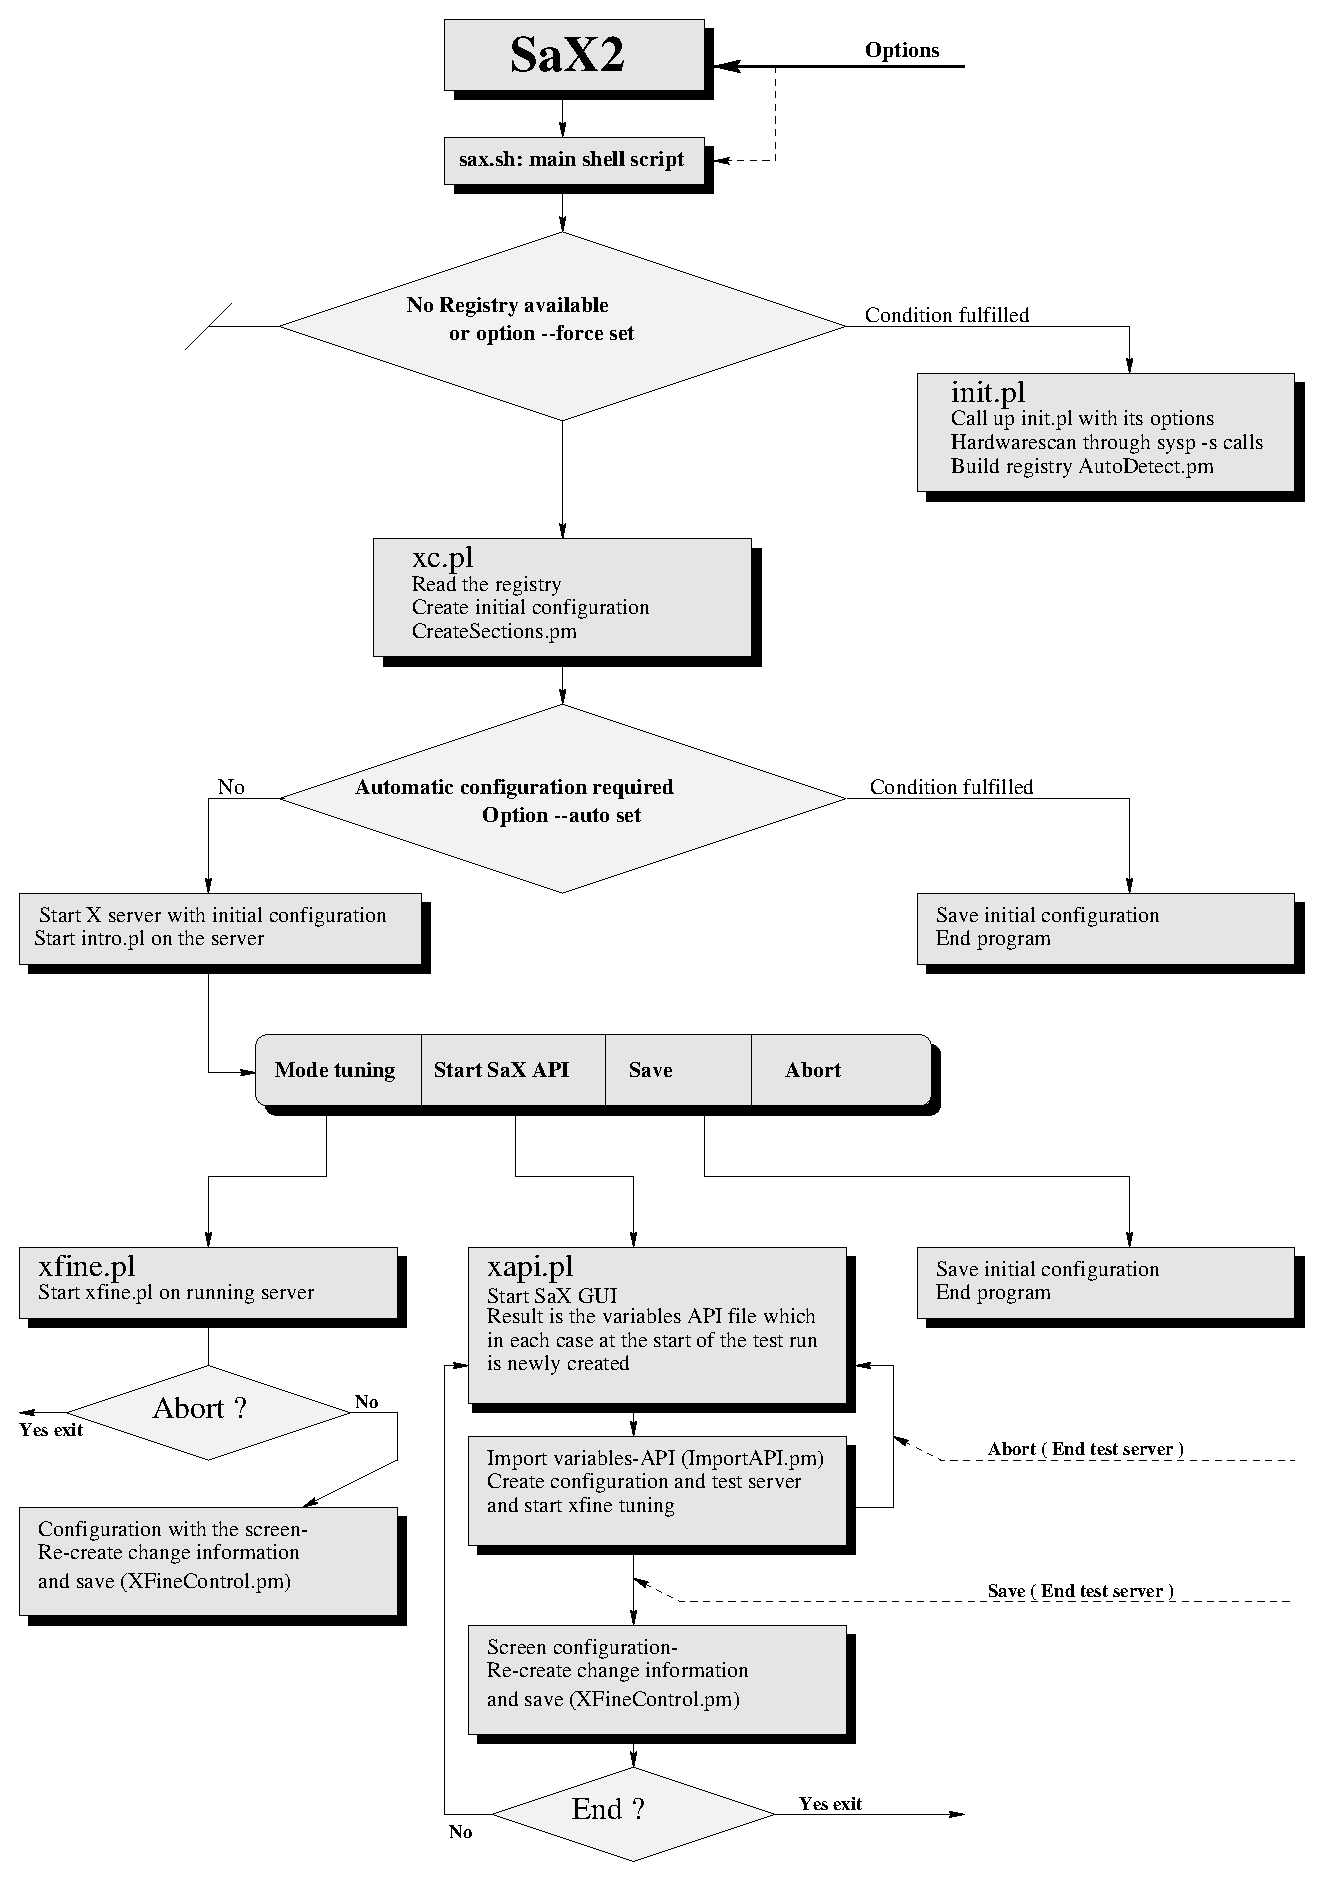
\epsfig{file=pictures/cheme.ps,width=10cm,height=16.5cm}
\caption{Flussdiagramm SaX2}
\end{figure}
